\Chapter{Tervezés}

A dolgozat által vizsgált témahoz egy komplex multifunkciós szoftver került megterve\hyp{}zésre, mely a dolgozati téma elemzési részében kifejezetten nagy szerepet tölt be. Összetettsége révén rengeteg időt és odafigyelést igényelt már maga a tervezési fázis is. Számos ábra és tervezet került megalkotásra, melynek a túlnyomó része rendkívül jelentősnek bizonyult az implementáció során.

A legmagasabb szinten az alábbi ábra nyújtja a legtisztább áttekintését a különböző funkcióknak és a szoftver sokszínűségének.

\begin{figure}[h!]
\begin{center}
\caption{\textbf{High-level áttekintő ábra}}
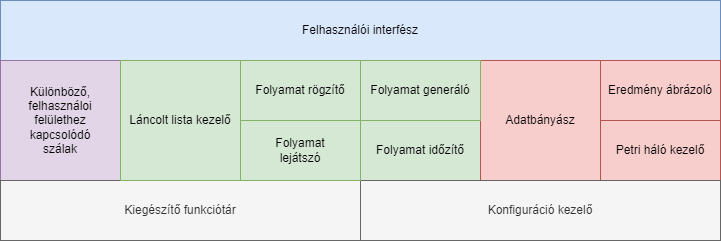
\includegraphics[width=\textwidth,keepaspectratio=true]{images/img_plan_1}
\label{fig:plan}
\end{center}
\end{figure}

\begin{itemize}
	\item \textbf{Felhasználói interfész}: A kezelőfelület, amivel a felhasználó eléri és kezelni tudja az egyes szoftverfunkciókat.
	\item \textbf{Felhasználói felülethez kapcsolódó szálak}: Fontos - a felhasználó számára nem látható - szálak, amelyek feldata bizonyos billentyűkombinációk figyelése anélkül, hogy a program reszponzivitását kártékonyan befolyásolnák.
	\item \textbf{Láncolt lista kezelő}: Az egyes folyamatok láncolt listaként vannak kezelve a szoftverbe, ez az alrendszer felel a megfelelő értelmezésükért. 
	\item \textbf{Folyamat rögzítő}: Figyeli és rögzíti a perifériák általi beviteli értékeket.
	\item \textbf{Folymat generáló}: Előre meghatározott forgatóvkönyvek alapján úgy generál folyamatokat mintha azt egy felhasználó végezte volna el.
	\item \textbf{Folyamat lejátszó}: A folyamatokat játsza vissza, egy felhasználót szimulál.
	\item \textbf{Folyamat időzítő}: A Windowsba integrált rendszert felhasználva ütemez / időzít folyamatokat.
	\item \textbf{Adatbányász}: Az Alpha-algoritmust implementálva folyamatelemzést hajt végre több folyamaton.
	\item \textbf{Eredmény ábrázoló}: Az Adatbányász által elvégzett folyamatelemzés eredmé\hyp{}nyeit jeleníti meg.
	\item \textbf{Petri háló kezelő}: A petri-hálót mint struktúra, valamint a hozzátartozó függvé\hyp{}nyeket a szoftver számára értelmezhető módon implementálja.
	\item \textbf{Kiegészítő funkciótár}: Számos hasznos funkció gyűjteménye, melyet a többi alrendsze használ.
	\item \textbf{Konfiguráció kezelő}: Futásidők között felhasználói preferenciák és beállítások tárolásáért és betöltéséért felel.
\end{itemize}

\Section{Az Alpha-algoritmus}

Az Alpha-algoritmust mint folyamatelemzési módszert hasznosan lehet alkalmazni a dolgozati témában. Az algoritmus, jelentőségét tekintve elengedhetetlen részét képezi a dolgozatnak. Jelen esetben a folyamatokat azok jellegétől és céljától függetlenül lehet elemezni, akár cél nélküli beviteli sorozatra is alkalmazható az Alpha-algoritmus.

\subsection{Alkalmazása}

Ebben az alfejezetben bemutatásra kerül, hogy hogyan is kapcsolódik pontosan az Alpha-algoritmus a dolgozat témájához.

Először is pontosan meg kell határozni, hogy milyen lépésekből áll az algoritmus.

\begin{definition}{\textit{($\alpha$-algoritmus):}} Legyen $L$ egy eseménynapló adott $E$ események hal\hyp{}maza felett. Ekkor a kimeneti $\alpha (L)$ petri hálót az alábbi módon határozzuk meg:
\begin{enumerate}
	\item Definiáljuk az összes eseményt.\\
	\[
		E_L = \{ e \in E | \exists_{\sigma \in L} e \in \sigma \},
	\]
	\item Definiáljuk az összes bemeneti eseményt.
	\[
		E_I = \{ e \in E | \exists_{\sigma \in L} e = first(\sigma) \},
	\]
	\item Definiáljuk az összes kimeneti eseményt.
	\[
		E_O = \{ e \in E | \exists_{\sigma \in L} e = last(\sigma) \},	
	\]
	\item Kiszámítjuk az összes lehetséges $A$ és $B$ halmazt úgy, hogy az összes esemény $A$-ban és $B$-ben függetlenek legyenek egymástól, valamint minden $A$-beli esemény okozati kapcsolatban álljon $B$-beli eseményekhez.
	\begin{equation*}
	\begin{aligned}
		X_L=
		&\{ (A,B) | A \subseteq E_L \land A \neq \emptyset \land B \subseteq E_L \land B \neq \emptyset \land \\
		&\forall_{a \in A} \forall_{b \in B} a \rightarrow_L b \land \forall_{a1,a2 \in A} a_1\#_L a_2  \land \forall_{b1,b2 \in B} b_1\#_Lb_2\},
	\end{aligned}
	\end{equation*}
	\item Elhagyjuk a nem-maxmiális halmazokat.
	\[
		Y_L = \{ (A,B) \in X_L | \forall_{A',B' \in X_L} A \subseteq A' \land B \subseteq B' \Rightarrow (A,B) = (A',B') \},
	\]
	\item Helyeket rendelünk az összes származtatott halmazhoz valamint a kezdő- és végál\hyp{}lapotokhoz.
	\[
		P_L = \{ p_{A,B} | (A,B) \in Y_L\} \cup \{i_L,o_L\},		
	\]
	\item Berajzoljuk a kapcsolatokat.
	\begin{equation*}
	\begin{aligned}
		F_L=
		&\{(a,p_{(A,B)} | (A,B) \in Y_L \land a \in A \} \cup \{ (p_{(A,B)}, b) | (A,B) \in \\
		&Y_L \land b \in B \} \cup \{ (i_L,e) | e \in E_I \} \cup \{ (e,o_L) | e \in E_O\},
	\end{aligned}
	\end{equation*}
	\item Visszatérünk a petri hálóval.
	\[
		\alpha(L) = (P_L, E_L, F_L).
	\]

\end{enumerate}

\textit{Forrás: \cite{article:001}}
\end{definition}

\begin{example}
	Ebben a példában három előre létrehozott folyamaton kerül alkalmazásra az Alpha-algoritmus. A folyamatok egyszerűek, hogy szemléletes legyen a példa, viszont ugyanezzel a módszerrel több száz vagy akár több ezer hosszú folyamaton is alkalmazha\hyp{}tó az algoritmus.
	
	Maguk a folyamatok szolgálnak bemenetként, részeredményekként eseménynapló és lenyomati mátrix jön létre, kimentként pedig egy olyan petri háló kerül generálásra mely leírja a folyamat modelljét.
	
	\begin{figure}[h]
	\begin{center}
	\caption{Beviteli folyamatok}
	\begin{tabular}{|| c | c | c | c | c | r ||}
		\hline\hline
		\textbf{Folyamat} & \textbf{ID} & \textbf{Típus} & \textbf{Érték} & \textbf{Érték típusa} &  \textbf{Eltelt idő} \\ [0.5ex]
		\hline\hline
		1 & 1 & Key&  Left Alt & WM\_SYSKEYDOWN & 0 \\
		\hline
		1 & 2 & Key&  F4 & WM\_SYSKEYDOWN & 100 \\
		\hline
		1 & 3 & Key&  F4 & WM\_SYSKEYUP & 150 \\
		\hline
		1 & 4 & Key&  Left Alt & WM\_KEYUP & 612 \\
		\hline\hline
		2 & 1 & Key & Left Alt & WM\_SYSKEYDOWN & 0 \\
		\hline
		2 & 2 & Key & F4 & WM\_SYSKEYUP & 80 \\
		\hline
		2 & 3 & Key & F4 & WM\_SYSKEYDOWN & 51 \\
		\hline
		2 & 4 & Key & Left Alt & WM\_KEYUP & 152 \\
		\hline\hline
		3 & 1 & Key & Left Alt & WM\_SYSKEYDOWN & 0 \\
		\hline
		3 & 2 & Mouse & 25:1022 & WM\_LBUTTONDOWN & 151 \\
		\hline
		3 & 3 & Key & Left Alt & WM\_KEYUP & 188 \\
		\hline\hline
	\end{tabular}
	\label{fig:planexample}
	\end{center}
	\end{figure}	
	
	Az Alpha-algoritmus alkalmazásában, mint bármely folyamatbányászati algorit\hyp{}musnál, első lépésként ezekből az eseményekből fel kell építeni az eseménynaplót amiből később dolgozik az algoritmus. Ez a lépés konkrétan arról szól, hogy a már meglévő folyamatok az Alpha-algoritmusnak szükséges formátumra kerülnek átalakításra.
	
	Ez jelen esetben az alábbi három szabály alapján történik:
	\begin{enumerate}
		\item A "\textbf{Folyamat}" elnevezésű oszlop alapján triviális módon meghatározásra kerül az esethez tartozó egyedi azonosító,
		\item A "\textbf{Típus}", "\textbf{Érték}" és "\textbf{Érték típusa}" oszlophármas értékeiből létrejön a tevékenység megnevezése,  ami a továbbiakban \textit{,,$T_{n}$"}-ként lesz feltüntet\hyp{}ve,
		\item Az "\textbf{Eltelt idő}" oszlop alapján (az előző esemény óta eltelt időt mutatja) pedig létrejön egy relatív-időbélyeg az "\textbf{ID}" oszlop segítségével, hiszen az utóbbi alap\hyp{}ján határozható meg az események szekvenciája.
	\end{enumerate}
	
	Ezeknek megfelelően az alábbi eseménynaplót kapjuk:
	
	\begin{figure}[h]
	\begin{center}
	\caption{Eseménynapló}
	\begin{tabular}{|| c | c | c ||}
		\hline
		Azonosító & Tevékenység & Relatív időbélyeg \\ [0.5ex]
		\hline\hline
		1 & $T_0$ & 0 \\
		\hline
		1 & $T_1$ & 100 \\
		\hline
		1 & $T_2$ & 250 \\
		\hline
		1 & $T_3$ & 762 \\
		\hline
		2 & $T_0$ & 0 \\
		\hline
		2 & $T_2$ & 80 \\
		\hline
		2 & $T_1$ & 131 \\
		\hline
		2 & $T_3$ & 283 \\
		\hline
		3 & $T_0$ & 0 \\
		\hline
		3 & $T_4$ & 151 \\
		\hline
		3 & $T_3$ & 339 \\
		\hline
	\end{tabular}
	\label{fig:planexample}
	\end{center}
	\end{figure}	
	
	Miután megvan az eseménynapló, a következő két lépésben meghatározzuk a beme\hyp{}neti- és kimeneti események halmazait:
	\begin{enumerate}
		\item $E_I=<T_0>$
		\item $E_O=<T_3>$		
	\end{enumerate}

\newpage
	Ezután a következő lépéshez az eseménynaplóban szereplő események kapcsolatait közvetlen-sorrend, okozat, párhuzam és választás relációkra alakítja az algoritmus.

	Ezzel jön létre az alábbi lenyomati mátrix:
	
	\begin{figure}[h]
	\begin{center}
	\caption{Lenyomati mátrix}
	\begin{tabular}{|c | c | c | c | c | c|}
		\hline
		\hspace{0.1cm} & $T_0$ & $T_1$ & $T_2$ & $T_3$ & $T_4$ \\
		\hline
		$T_0$ & \# & $\rightarrow$ & $\rightarrow$ & \# & $\rightarrow$ \\
		\hline
		$T_1$ & $\leftarrow$ & \# & $\parallel$ & $\rightarrow$ & \# \\
		\hline
		$T_2$ & $\leftarrow$ & $\parallel$ & \# & $\rightarrow$ & \# \\
		\hline
		$T_3$ & \# & $\leftarrow$ & $\leftarrow$ & \# & $\leftarrow$ \\
		\hline
		$T_4$ & $\leftarrow$ & \# & \# & $\rightarrow$ & \# \\
		\hline
	\end{tabular}
	\label{fig:planexample}
	\end{center}
	\end{figure}

	Ezen a mátrixon kerül ábrázolásra az összes esemény közötti kapcsolat. Több szem\hyp{}pontból is hasznos ez a mátrix, többek között a struktúrája is megfelelő ahhoz, hogy program szinten meghatározzuk a következő lépésben a lehetséges halmazpárokat, vala\hyp{}mint emberi szemmel is kifejezetten könnyen értelmezhető.

	Ezt a mátrixot felhasználva az alábbi halmazpárok lehetségesek a jelenlegi példában:

	\begin{figure}[h]
	\begin{center}
	\caption{Lehetséges halmazpárok}
	\begin{tabular}{|| c | c ||}
		\hline
		A & B \\
		\hline\hline
		\{$T_0$\} & \{$T_1$\} \\
		\hline
		\{$T_0$\} & \{$T_2$\} \\
		\hline
		\{$T_0$\} & \{$T_4$\} \\
		\hline
		\{$T_1$\} & \{$T_3$\} \\
		\hline
		\{$T_2$\} & \{$T_3$\} \\
		\hline
		\{$T_4$\} & \{$T_3$\} \\
		\hline
		\{$T_0$\} & \{$T_1, T_4$\} \\
		\hline
		\{$T_0$\} & \{$T_2, T_4$\} \\
		\hline
		\{$T_1, T_4$\} & \{$T_3$\} \\
		\hline
		\{$T_2, T_4$\} & \{$T_3$\} \\
		\hline
	\end{tabular}
	\label{fig:planexample}
	\end{center}
	\end{figure}	

\newpage
	Következő lépésként ezekből a halmazpárokból kell eltávolítani a nem-maximálisak\hyp{}at, azaz azokat amik részhalmazai egy másiknak. Ezt program szinten egy többszörös ciklus segítségével könnyedén el lehet végezni, jelen példában pedig az alábbi négy halmazpár maradt:
	
	\begin{figure}[h]
	\begin{center}
	\caption{Maradék halmazpárok}
	\begin{tabular}{|| c | c ||}
		\hline
		A & B \\
		\hline\hline
		\{$T_0$\} & \{$T_1, T_4$\} \\
		\hline
		\{$T_0$\} & \{$T_2, T_4$\} \\
		\hline
		\{$T_1, T_4$\} & \{$T_3$\} \\
		\hline
		\{$T_2, T_4$\} & \{$T_3$\} \\
		\hline
	\end{tabular}
	\label{fig:planexample}
	\end{center}
	\end{figure}

	Miután ezek a halmazpárok meghatározásra kerültek, helyek $(p_1-p_4)$  lesznek hozzájuk rendelve. Ezekhez a helyekhez létrehozásra kerülnek a megfelelő bemeneti és kimeneti átmenetek, valamint a végső bemeneti és kimeneti állapotok is.

	Amint ez megvan, berajzolásra kerülnek a kapcsolatok is, a végén pedig a következő petri háló kerül megjelenítésre.

	\begin{figure}[h!]
	\begin{center}
	\caption{\textbf{Kimeneti petri háló}}
	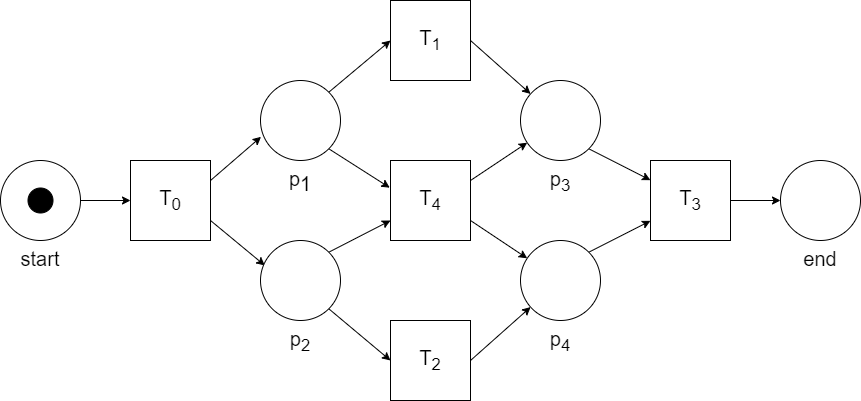
\includegraphics[width=\textwidth,keepaspectratio=true]{images/img_plan_2}
	\label{fig:plan}
	\end{center}
	\end{figure}


\end{example}























